%% if you are submitting an initial manuscript then you should have submission as an option here
%% if you are submitting a revised manuscript then you should have revision as an option here
%% otherwise options taken by the article class will be accepted
\documentclass[submission]{FPSAC2025}
%% but DO NOT pass any options (or change anything else anywhere) which alters page size / layout / font size etc

%% note that the class file already loads {amsmath, amsthm, amssymb}

\newtheorem{thm}{Theorem}
\newtheorem{conj}{Conjecture}
\newtheorem{cor}{Corollary}
\newtheorem{lem}{Lemma}

\usepackage{lipsum,mathtools,tikz}

\newcommand{\dfemph}[1]{\textcolor{blue}{\emph{#1}}}

\DeclareMathOperator{\gr}{gr}
\DeclareMathOperator{\tr}{tr}

\newcommand{\id}{\mathrm{id}}
\newcommand{\m}{p}
\newcommand{\x}{\mathbf{v}}

\newcommand{\Asc}{\mathrm{Asc}}
	\newcommand{\Des}{\mathrm{Des}}
\newcommand{\Br}{\mathit{Br}}
\newcommand{\HOMFLYPT}{\mathcal{P}}
\newcommand{\HHH}{\mathrm{HHH}}
\newcommand{\Cat}{\mathrm{Cat}}
\newcommand{\CharQ}[1]{\chi_{q, #1}}
\newcommand{\Park}{\mathrm{Park}}
\newcommand{\ParkSpace}{\Pi}

%% define your title in the usual way
\title{Cell Decompositions of Hecke Traces and Link Polynomials}

%HOMFLY Coefficients via Cell Decompositions \\
%and Parabolic $W$-Parking Combinatorics


%% define your authors in the usual way
%% use \addressmark{1}, \addressmark{2} etc for the institutions, and use \thanks{} for contact details
%% for more than 3 names, use the Oxford comma: One Author, Two Author, Red Author, \and Blue Author
\author{Minh-T\^{a}m Quang Trinh\thanks{\href{mailto:minh-tam.trinh@yale.edu}{minh-tam.trinh@yale.edu}. M.\ Q.\ Trinh was partially supported by an NSF Mathematical Sciences Research Fellowship, Award DMS-2002238.}\addressmark{1} \and Nathan Williams\thanks{\href{mailto:nathan.f.williams@gmail.com}{nathan.f.williams@gmail.com}. N. Williams was partially supported by NSF Grant DMS-2246877.}\addressmark{2}}

%% then use \addressmark to match authors to institutions here
\address{\addressmark{1}Department of Mathematics, Yale University, New Haven, CT 06520 \\ \addressmark{2}Mathematical Sciences Department, University of Texas at Dallas, Richardson, TX 75080}

%% put the date of submission here
\received{November 15, 2024}

%% leave this blank until submitting a revised version
%\revised{}

%% put your English abstract here, or comment this out if you don't have one yet
%% please don't use custom commands in your abstract / resume, as these will be displayed online
%% likewise for citations -- please don't use \cite, and instead write out your citation as something like (author year)
\abstract{For specific trace functions on the Hecke algebra of a finite Weyl group $W$, we establish formulas for their values at positive braids in terms of point counts of Deodhar-type cells in associated algebraic varieties.
For irreducible $W$, we deduce a uniform enumeration result that interpolates between its rational Catalan and parking combinatorics, generalizing our earlier work with Galashin and Lam.
The key is a new relationship between the varieties from that work and the braid Steinberg varieties introduced by Trinh.
For $W = S_n$, we prove a similar point-counting formula for each $a$-degree in the HOMFLYPT polynomial of the link closure of the braid, generalizing work of Shende--Treumann--Zaslow for the ``highest'' degree.
}

%% put your French abstract here, or comment this out if you don't have one
%\resume{}

%% put your keywords here, or comment this out if you don't have them yet
\keywords{Hecke algebra, link invariant, Coxeter--Catalan combinatorics, Deodhar cell, braid variety, Springer fiber}

%% you can include your bibliography however you want, but using an external .bib file is STRONGLY RECOMMENDED and will make the editor's life much easier
%% regardless of how you do it, please use numerical citations; i.e., [xx, yy] in the text

%% this sample uses biblatex, which (among other things) takes care of URLs in a more flexible way than bibtex
%% but you can use bibtex if you want
\usepackage[backend=bibtex]{biblatex}
\addbibresource{norms_fpsac.bib}
%% note the \printbibliography command at the end of the file which goes with these biblatex commands

\begin{document}

\maketitle

\section{Introduction}

In this work, we present a collection of formulas for special values of special traces on the Hecke algebras $H_W(\x)$ associated with finite Weyl groups $W$.
These formulas arise from point counting on algebraic varieties over finite fields.
Nonetheless, the traces subsume various polynomials studied in combinatorics and knot theory: in the former, polynomials interpolating between the rational $q$-Catalan and parking numbers of $W$; in the latter, \emph{arbitrary} $a$-degrees of the HOMFLYPT polynomials of positive links.

The role of Hecke algebras in both subjects is well-known.
Our new contribution is to focus attention on central elements of the form
\begin{align}
\sum_{w \in X} \sigma_w \sigma_{w^{-1}},
\end{align}
where $X$ is a subset of $W$, and $(\sigma_w)_{w \in W}$ denotes the standard basis of the Hecke algebra in a particular normalization.
These central elements interact nicely with certain cell decompositions of our algebraic varieties, which generalize and take inspiration from similar decompositions studied by Deodhar~\cite{deodhar}.

In the rest of this introduction, we review all necessary background.
In Section \ref{sec:varieties}, we introduce various algebraic varieties associated with positive elements in the braid group of $W$, and state our results about their cell decompositions.
In Section \ref{sec:traces}, we state applications to relative norms for Hecke algebras, link invariants, and combinatorial enumeration, as well as some directions of ongoing work.
Throughout, we use the standard ``$q$-notations'' $[k]_q \vcentcolon= 1 + q + \cdots + q^{k - 1}$ and $[k]_q! \vcentcolon= [k]_q \cdots [2]_q[1]_q$.

\subsection{HOMFLYPT and Catalan}

The relationship between algebraic geometry, knot theory, and Catalan combinatorics can be traced back to a link invariant discovered in the 80s, now called the \dfemph{(reduced) HOMFLYPT polynomial}~\cite{homfly}:
\begin{align}
\HOMFLYPT : \{\text{links in $\mathbb{R}^3$}\}/\text{isotopy} \to \mathbb{Z}[a^{\pm 1}](\x).
\end{align}
On the one hand, pieces of the HOMFLYPT polynomials of certain links, called torus knots, recover $q$-analogues of the \dfemph{rational Catalan numbers} defined by
\begin{align}
\Cat_{n, \m} = \frac{(\m + n - 1)!}{n!\m!}
	\quad\text{for all coprime $n, \m > 0$},
\end{align}
which themselves recover the classical Catalan numbers at $\m = n + 1$; explicitly, the \dfemph{rational $q$-Catalan number} $\Cat_{n, \m}(q)$ is defined by replacing each factorial $k!$ above with $[k]_q!$.
On the other hand, the HOMFLYPT polynomials of links more general than torus knots can be expressed in terms of the point counts of certain algebraic varieties built from the groups $\mathrm{GL}_n(\mathbb{F}_q)$ and their flag varieties.
%Our work extends the resulting bridge between $q$-Catalan numbers and these varieties to other families of $q$-numbers; from $\mathrm{GL}_n(\mathbb{F}_q)$ to other groups; and most importantly, to meaningful combinatorics in the $q \to 1$ limit.

The phenomena described above were discovered through a particular construction of HOMFLYPT due to Ocneanu. 
First recall the fact, due to Alexander, that every link is the closure of some \dfemph{braid} $\beta$ up to isotopy.
In this case we denote the link isotopy class by $L_\beta$.
From the braid group on $n$ strands 
\begin{align}
\Br_n = \left\langle \sigma_1, \ldots, \sigma_{n - 1}\, \middle|
	\begin{array}{r@{\:}ll}
	\sigma_i \sigma_{i + 1} \sigma_i
		&= \sigma_{i + 1} \sigma_i \sigma_{i + 1}
		&\text{for $1 \leq i \leq n - 2$},\\
	\sigma_i \sigma_j
		&= \sigma_j \sigma_i
		&\text{for $|i - j| > 1$}
	\end{array}
	\right\rangle,
\end{align}
or rather, its group algebra over $\mathbb{Z}[\x^{\pm 1}]$, one constructs the \dfemph{Hecke algebra} 
\begin{align}
H_n(\x) = \frac{\mathbb{Z}[\x^{\pm 1}]\Br_n}{\langle \text{$(\sigma_i - \x)(\sigma_i + \x)$ for all $i$}\rangle}.
\end{align}
A \dfemph{trace} on $H_n(\x)$ is a $\mathbb{Z}[\x^{\pm 1}]$-linear function that takes the same value on $\alpha\beta$ and $\beta\alpha$ for all $\alpha, \beta \in H_n(\x)$.
Ocneanu constructed such a trace $\xi_n : H_n(\x) \to \mathbb{Z}[a^{\pm 1}](\x)$ for all $n$, and showed how to construct $\HOMFLYPT(L_\beta)$ for all $\beta \in \Br_n$ by renormalizing $\xi_n(\beta)$~\cite{jones-v}.

The Hecke algebra, in turn, specializes at $\x \to 1$ to the group ring $\mathbb{Z}S_n$.
Through the close connection between the representation theories of $H_n(\x)$ and $S_n$, Jones computed the HOMFLYPT polynomial of the \dfemph{$(n, \m)$-torus knot} $L_{n, \m} \vcentcolon= L_{(\sigma_1 \cdots \sigma_{n - 1})^\m}$, for $\m > 0$ coprime to $n$~\cite{jones-v}.
In modern conventions, the powers of $a$ in this polynomial range between $\mu$ and $\mu + 2(\min(n, \m) - 1)$, where $\mu = (n - 1)(\m - 1)$.

For a general link $L$, it will be convenient to write $\HOMFLYPT_i(L)$ for the $\mathbb{Z}[\x^{\pm 1}]$-coefficient of $a^{\mathrm{low} + i}$ in $\HOMFLYPT(L)$, where $a^\mathrm{low}$ is the lowest power of $a$ occurring in $\HOMFLYPT(L)$.
Inspection of Jones's formula shows a relationship to rational $q$-Catalan numbers:
\begin{align}\label{eq:jones}
\x^{-\mu} \Cat_{S_n, \m}(\x^2)
	&= \HOMFLYPT_0(L_{n, \m})
	= \HOMFLYPT_{2(n - 1)}(L_{n, \m + n}).
\end{align}
%However, his proof does not give an enumerative explanation for their appearance.

\subsection{Geometry over $\mathbb{F}_q$}\label{subsec:geo}

It turns out that the algebras $H_n(\x)$ do have an enumerative meaning that involves their relation to the groups $G = \mathrm{GL}_n(\mathbb{F}_q)$.
To explain, fix a \dfemph{Borel subgroup} $B \subseteq G$, such as the subgroup of upper-triangular matrices, and recall the Bruhat decomposition
\begin{align}
G = \coprod_{w \in S_n} BwB,
\end{align}
where each element of $S_n$ has been lifted to a permutation matrix in $G$.
By a classical theorem of Iwahori, $H_n(q^{1/2}) \vcentcolon= H_n(\x)|_{\x = q^{1/2}}$ is isomorphic to a certain convolution algebra formed by $(B \times B^\mathrm{op})$-invariant functions on $G$.
%\cite{iwahori} 
%\cite[Ch.\ 2]{carter}.

The quotient $G/B$ can be identified with the set of complete flags in $\mathbb{F}_q^n$.
Iwahori's result can be rewritten in terms of $G/B$ as follows.
First, a pair of cosets $(yB, xB)$ is said to be in \dfemph{relative position} $w \in S_n$ if and only if $By^{-1}xB = BwB$.
In this case, we write $yB \xrightarrow{w} xB$.
The stratification of $G/B \times G/B$ by relative position is precisely its stratification into orbits under the diagonal action of $G$.
Thus $H_n(q^{1/2})$ also forms a convolution algebra of $G$-invariant functions on $G/B \times G/B$.
The indicator functions of the $G$-orbits lift to the elements of a basis for $H_n(\x)$ as a free module over $\mathbb{Z}[\x^{\pm 1}]$, called the \dfemph{standard basis} $\{\mathbf{1}_w\}_{w \in S_n}$.

In our conventions, $\sigma_i = \x^{-1}\mathbf{1}_{s_i}$, where $s_i = (i, i + 1) \in S_n$.
Fix a word $\vec{s} = (s_{i_1}, \ldots, s_{i_\ell})$ and set $\beta_{\vec{s}} = \sigma_{i_1} \cdots \sigma_{i_\ell} \in \Br_n$.
In~\cite{stz}, Shende--Treumann--Zaslow observed that
\begin{align}\label{eq:stz}
\frac{|X(\vec{s})|}{|G|} = \left.\left[\x^{\ell - n}\,\HOMFLYPT_{2(n - 1)}(L_{\beta_{\vec{s}}})\right]\right|_{\x \to q^{1/2}},
\end{align}
where the left-hand side uses the set
\begin{align}
X(\vec{s}) = \{(x_1B, \ldots, x_\ell B) \in (G/B)^\ell \mid x_\ell B \xrightarrow{s_{i_1}} x_1 B \xrightarrow{s_{i_2}} \cdots \xrightarrow{s_{i_\ell}} x_\ell B\}.
\end{align}
Their original proof involved a partition of $X(\vec{s})$ into subsets indexed by so-called rulings of a Legendrian representative of $L_{\beta_{\vec{s}}}$.
We now know a more direct proof.
The main step is to show that $|X(\vec{s})| = \tau(\beta_{\vec{s}})|_{\x \to q^{1/2}}$, where $\tau : H_n(\x) \to \mathbb{Z}[\x^{\pm 1}]$ is the trace given by 
\begin{align}\label{eq:tau}
\tau(\mathbf{1}_\id) = 1
	\quad\text{and}\quad
\tau(\mathbf{1}_w)
	= \text{$0$ for $w \neq \id$}.
\end{align}
In what follows, let $\mathbf{G}, \mathbf{B}, \mathbf{X}(\vec{s})$ be the algebraic groups and varieties over $\bar{\mathbb{F}}_q$ that recover $G, B, X(\vec{s})$ on Frobenius-fixed points.
Here we use the Frobenius map $F : \mathbf{G} \to \mathbf{G}$ given on matrix coordinates $x_{i,j}$ by $F(x_{i,j}) = x_{i,j}^q$.
Note that the $\mathbf{G}$-action on $\mathbf{G}/\mathbf{B}$ induces a $\mathbf{G}$-action on $\mathbf{X}(\vec{s})$.

In the mid-2000s, Khovanov--Rozansky discovered a link invariant now called \dfemph{triply-graded link homology} and denoted $\HHH$, whose (triply)-graded dimension is a refinement of $\HOMFLYPT$.
Let $\HHH_i \subseteq \HHH$ be the summand corresponding to $\HOMFLYPT_i$.
In~\cite{gl}, Galashin--Lam strengthened \eqref{eq:stz} for so-called Richardson braids $\beta_{\vec{s}}$, by matching $\HHH_{2(n - 1)}(L_{\beta_{\vec{s}}})$ with the weight-graded, $\mathbf{G}$-equivariant compactly-supported cohomology of $\mathbf{X}(\vec{s})$.
It is explained there that when $L_{\beta_{\vec{s}}} = L_{n, \m}$, the cohomological and weight gradings recover the \dfemph{rational $q, t$-Catalan number} $\Cat_{n, \m}(q, t)$ studied by Loehr--Warrington, Hikita, and others, via a Dyck-path formula for $\HHH(L_{n, \m})$ conjectured by Gorsky--Negu\c{t} 
%\cite{gn} 
and proved by Mellit.
These $q, t$-numbers specialize to our $q$-numbers.
%In our conventions,
%\begin{align}
%C_{S_n, m}(q) = q^{(m - 1)(n - 1)/2} C_{n, m}(q, q^{-1}).
%\end{align}

Later, for general $\vec{s}$, Trinh proved a formula for the entire triply-graded homology $\HHH(L_{\beta_{\vec{s}}})$, in terms of an $S_n$-action on the weight-graded, $\mathbf{G}$-equivariant cohomology of a larger \dfemph{Steinberg variety} $\mathbf{Z}(\vec{s})$.
Taking the anti-invariant part of the formula gives an extension of the Galashin--Lam result to all $\vec{s}$~\cite{trinh_21}.
For our purposes, we only need a more elementary construction that produces a \emph{rational} character of $S_n$ depending on $q$, which we will define in \S\ref{subsec:springer} and denote by $\CharQ{\mathbf{Z}(\vec{s})} : \mathbb{Q}S_n \to \mathbb{Q}$.

\begin{thm}[Trinh~\cite{trinh_21}]\label{thm:trinh-homflypt}
For any word $\vec{s}$, we have $\HOMFLYPT(L_{\beta_{\vec{s}}})|_{\x \to q^{1/2}} = \sum_k {(-a^2)^k}\CharQ{\mathbf{Z}(\vec{s})}(e_{S_n, \Lambda^k})$, where the elements $e_{S_n, \Lambda^k} \in \mathbb{Q}S_n$ are defined in \S\ref{subsec:kirkman}.
\end{thm}

\subsection{From $S_n$ to $W$}\label{subsec:weyl}

The varieties above generalize beyond $\mathbf{G} = \mathbf{GL}_n$ to any (connected, smooth) reductive algebraic group $\mathbf{G}$ over $\bar{\mathbb{F}}_q$.
Any such algebraic group is determined by a root datum $(\Phi \subseteq \mathrm{X}, \Phi^\vee \subseteq \mathrm{X}^\vee)$, consisting of dual lattices $\mathrm{X}, \mathrm{X}^\vee$ and root systems $\Phi, \Phi^\vee$ satisfying certain conditions.
In this setting, the symmetric group $S_n$ is replaced by the \dfemph{Weyl group} $W$ of $\Phi$, a reflection group of the vector space $V \vcentcolon= \mathrm{X}^\vee \otimes \mathbb{Q}$.
The set of transpositions $\{s_i\}_i \subseteq S_n$ is replaced by a minimal generating set of \dfemph{simple reflections} $S \subseteq W$.
Thus, any word $\vec{s}$ in $S$ gives rise to a $\mathbf{G}$-variety $\mathbf{Z}(\vec{s})$ with a $W$-action on some version of its cohomology, and to a rational character $\CharQ{\mathbf{Z}(\vec{s})} : \mathbb{Q}W \to \mathbb{Q}$, also defined in \S\ref{subsec:springer}.

The pair $(W, S)$ forms an example of a finite Coxeter system.
% \cite[Ch.\ 2]{carter}.
This structure gives rise to a group $\Br_W$ generalizing $\Br_n$, and to an algebra $H_W(\x)$ generalizing $H_n(\x)$.
The analogue of $\sigma_1 \cdots \sigma_{n - 1} \in \Br_n$ is an element $\beta_{\vec{c}} \in \Br_W$, where $\vec{c}$ is a fixed ordering of $S$, or \dfemph{Coxeter word}.
In general, the elements of $\Br_W$ are no longer related to knot theory in the way that classical braids are.
%, Y.\@ Gomi constructed traces $\xi_W : H_W \to \mathbb{Z}[a^{\pm 1}](v)$ that uniformly generalize the traces $\xi_n : H_n \to \mathbb{Z}[a^{\pm 1}](v)$ introduced by Ocneanu.

By a classical theorem of Chevalley, the graded ring of invariants $\mathbb{Q}[V]^W$, where $V$ is placed in degree $1$, is freely generated by homogeneous elements.
Their degrees $d_1 \leq \cdots \leq d_r$, where $r = \dim V$, are called the \dfemph{(fundamental) degrees} of the $W$-action on $V$.
If $W$ is \dfemph{irreducible}, meaning it is not a direct product of two smaller reflection groups, then $d_r$ is the unique largest degree, called the \dfemph{Coxeter number} of $W$ and denoted $h$.
Coxeter--Catalan combinatorics studies enumerative interpretations of the \dfemph{rational Catalan numbers} of $W$, defined in the irreducible cases by
\begin{align}\label{eq:catalan}
\Cat_{W, \m} = \prod_{1 \leq i \leq r} \frac{\m + d_i - 1}{d_i}
	\quad\text{for all $\m > 0$ coprime to $h$}.
\end{align}
The \dfemph{rational $q$-Catalan number} $\Cat_{W, \m}(q)$ is formed by replacing the $i$th factor above with $[\m + d_i - 1]_q/[d_i]_q$.
It turns out that $\Cat_{W, \m}(q) \in \mathbb{Z}[q]$.
%, though this is not necessarily obvious.
When $W = S_n$, the fundamental degrees are $2, 3, \ldots, n$, giving $\Cat_{S_n, \m}(q) = \Cat_{n, \m}(q)$.

A major tool in this subject is a finite-dimensional graded representation of $W$ that we will call the \dfemph{(algebraic) rational parking space} and denote by $\ParkSpace_{W, \m} = \bigoplus_i \ParkSpace_{W, \m}^i$.
Its graded dimension is $[\m]_q^r$, the \dfemph{rational $q$-parking number}, whereas the graded dimension of its $W$-invariant subspace is the rational $q$-Catalan number $\Cat_{W, \m}(q)$.
By character theory, $\ParkSpace_{W, \m}$ is determined up to isomorphism by requiring that
\begin{align}\label{eq:trace-parking}
\sum_i q^i \tr(w \mid \ParkSpace_{W, \m}^i) = \frac{\det(1 - q^\m w \mid V)}{\det(1 - qw \mid V)}
	\quad\text{for all $w \in W$}.
\end{align}
%When $W = S_n$ and $\m = n + 1$, it is the module of diagonal coinvariants studied by Haiman~\cite{haiman}, Haglund~\cite{haglund}, and others, with its bigrading collapsed to a single grading.
%For general $W$ and
As explained in~\cite{arr}, it can be realized as a quotient of the polynomial ring $\mathbb{Q}[V]$ by an ideal depending on $\m$, arising from the representation theory of the so-called rational Cherednik algebra of $W$.
It can also be realized via the Steinberg varieties of~\cite{trinh_21}:

\begin{thm}[Trinh~\cite{trinh_21}]\label{thm:trinh-parking}
If $\vec{c}$ is a Coxeter word for $(W, S)$, and $\vec{c}^\m$ is its $\m$-fold concatenation, then $\CharQ{\mathbf{Z}(\vec{c}^\m)}(w)$ matches the expressions in \eqref{eq:trace-parking}.
\end{thm}

%We are led to seek a more direct relationship between $Z(\vec{c}^\m)$ and Coxeter--Catalan combinatorics.

\section{Cell Decompositions}\label{sec:varieties}

Henceforth, we reserve \textbf{boldface} uppercase for algebraic varieties and algebraic groups over $\bar{\mathbb{F}}_q$, and ordinary \emph{italics} for the corresponding sets and groups formed by their $F$-fixed points, where $F : \mathbf{G} \to \mathbf{G}$ is the Frobenius map arising from a split $\mathbb{F}_q$-form of $\mathbf{G}$.
We mention without further comment that some $q$-identities below require that the characteristic of $\mathbf{F}_q$ not divide $|W|$.

We fix an $F$-stable Borel subgroup $\mathbf{B} \subseteq \mathbf{G}$ and an $F$-stable, maximally split maximal torus $\mathbf{T} \subseteq \mathbf{B}$.
Once we identify $W$ with $N_\mathbf{G}(\mathbf{T})/\mathbf{T}$, we get a Bruhat decomposition of $\mathbf{G}$, \emph{resp.}\@ $G$, into double cosets $\mathbf{B}w\mathbf{B}$, \emph{resp.}\@ $BwB$.
(``Maximally split'' implies that $N_\mathbf{G}(\mathbf{T})/\mathbf{T} \simeq N_G(T)/T$.)
Note that $r = \dim \mathbf{T}$.

Recall that for any $w \in W$, the \dfemph{Bruhat length} $\ell(w)$ is the minimal length among words in $S$ that represent $w$, or equivalently, the dimension of $\mathbf{B}w\mathbf{B}/\mathbf{B}$.
%It turns out that $\ell(w) = \dim \mathbf{B}w\mathbf{B}/\mathbf{B}$.
The \dfemph{Bruhat order} on $W$ is the partial order $<$ generated by the relations $w < ws$ for all $w \in W$ and $s \in S$ such that $\ell(w) < \ell(ws)$, and the analogous relations with $sw$ in place of $ws$.
There is a unique, involutive, longest element $w_\circ \in W$; multiplication by $w_\circ$ inverts the Bruhat order.

\subsection{Richardson Varieties and Deodhar Cells}

As a warm-up, we review a simpler construction from our joint work with Galashin and Lam~\cite{gltw}.
For any word $\vec{s} = (s^{(1)}, \ldots, s^{(\ell)})$ in $S$, let
\begin{align}
\mathbf{O}(\vec{s}) = \{\vec{x}\mathbf{B} = (x_0\mathbf{B}, x_1\mathbf{B}, \ldots, x_\ell\mathbf{B}) \in (\mathbf{G}/\mathbf{B})^{1 + \ell} \mid x_0\mathbf{B} \xrightarrow{s^{(1)}} x_1\mathbf{B} \xrightarrow{s^{(2)}} \cdots \xrightarrow{s^{(\ell)}} x_1\mathbf{B}\}.
\end{align}
For any $v \in W$, the \dfemph{$v$-twisted (open) Richardson variety} of $\vec{s}$ in~\cite{gltw} is
\begin{align}
\mathbf{R}^{(v)}(\vec{s})
	= \{
		\vec{x}B \in \mathbf{O}(\vec{s}) \mid
		x_\ell \mathbf{B} \xrightarrow{vw_\circ} \mathbf{B} = x_0vw_\circ\mathbf{B}
		\}.
\end{align}
These varieties admit cell decompositions of the following form.

Recall that a \dfemph{subword} of $\vec{s}$ is a sequence $\vec{\omega} = (\omega^{(1)}, \ldots, \omega^{(\ell)})$ such that $\omega^{(i)} \in \{\id, s^{(i)}\}$ for all $i$.
It will be convenient to write $\omega_{(i)} \vcentcolon= \omega^{(1)} \cdots \omega^{(i)}$ below.
For any $v \in W$, a \dfemph{$v$-distinguished subword} of $\vec{s}$ is a subword $\vec{\omega}$ such that $v\omega_{(i)}  \leq v\omega_{(i - 1)} s^{(i)}$ for all $i$.
For any such $\vec{\omega}$, we set
\begin{align}
\mathbf{d}_{\vec{\omega}} = \{i \mid v\omega_{(i)} < v\omega_{(i - 1)}\}
	\quad\text{and}\quad
	\mathbf{e}_{\vec{\omega}} = \{i \mid \omega^{(i)} = \id\}.
\end{align}
Let $\mathcal{D}^{(v)}(\vec{s})$ be the set of $v$-distinguished subwords $\vec{\omega}$ of $\vec{s}$ for which $\smash{\omega_{(\ell)}} = \id$, and let $\mathcal{M}^{(v)}(\vec{s}) \subseteq \mathcal{D}^{(v)}(\vec{s})$ be the subset of $\vec{\omega}$ such that $|\mathbf{e}_{\vec{\omega}}| = r$.
Then Deodhar essentially observed in~\cite{deodhar} that $\mathbf{R}^{(v)}(\vec{s})$ is partitioned by disjoint, $\mathbf{B}$-stable subvarieties $\mathbf{R}^{(v)}(\vec{s}, \vec{\omega})$, now called \dfemph{Deodhar cells}, for $\vec{\omega}$ running over $\mathcal{D}^{(v)}(\vec{s})$ and
\begin{align}
\mathbf{R}^{(v)}(\vec{s}, \vec{\omega}) 
	&\vcentcolon= \{\vec{x}\mathbf{B} \in \mathbf{R}^{(v)}(\vec{s}) \mid \text{$\mathbf{B} \xrightarrow{w_\circ v\omega_{(i)}} x_i\mathbf{B}$ for all $i$}\}\\[0.5ex]
	&\simeq \left\{\vec{t} \in \mathbf{A}^\ell\, \middle|
		\begin{array}{ll}
		t_i \neq 0
			&\text{for $i \in \mathbf{e}_{\vec{\omega}}$},\\
		t_i= 0
			&\text{for $i \notin \mathbf{d}_{\vec{\omega}} \cup \mathbf{e}_{\vec{\omega}}$}
		\end{array}\!\right\}.
\end{align}
Above, $\mathbf{A}^\ell$ denotes $\ell$-dimensional affine space.
In particular,
\begin{align}\label{eq:deodhar}
|R^{(v)}(\vec{s}, \vec{\omega})| = q^{|\mathbf{d}_{\vec{\omega}}|} (q - 1)^{|\mathbf{e}_{\vec{\omega}}|}.
\end{align}
This relates the point count $|R^{(v)}(\vec{s})|$ to the trace \eqref{eq:tau}, since we showed in~\cite{gltw} that
\begin{align}\label{eq:gltw}
\tau(\beta_{\vec{s}} \sigma_{vw_\circ} \sigma_{(vw_\circ)^{-1}}) 
= 
	\sum_{\vec{\omega} \in \mathcal{D}^{(v)}(\vec{s})}
	\x^{2|\mathbf{d}_{\vec{\omega}}|} (\x^2 - 1)^{|\mathbf{e}_{\vec{\omega}}|},
\end{align}
where, for all $w \in W$, we have set $\sigma_w = \x^{-\ell(w)} \mathbf{1}_w$.
Indeed, when $W = S_n$, the Deodhar cell decomposition recovers the ruling partition mentioned in \emph{loc.\@ cit.}

%\begin{thm}[Deodhar]
%We can partition $\bb{R}^{(v)}(\vec{s})$ into disjoint subvarieties $\bb{R}^{(v)}(\vec{s}, \vec{x})$ running over $\vec{x} \in \sf{D}^{(v)}(\vec{s})$, where
%\begin{align}
%\bb{R}^{(v)}(\vec{s}, \vec{x}) 
%	= \{\vec{x}B \in \bb{R}^{(v)}(\vec{s}) \mid \text{$B_+ \xrightarrow{w_\circ vx_{(i)}} B_i$ for all $i$}\}.
%\end{align}
%These subvarieties are $(B_{+, w_\circ v} \times F)$-stable.
%For each $\vec{x}$, there is an $F$-equivariant isomorphism $\bb{A}^{\sf{d}_v(\vec{x})} \times \bb{G}^{\sf{e}_v(\vec{x})} \xrightarrow{\sim} \cal{R}_{\vec{s}}(\vec{x})$, where
%\begin{align}
%\bb{A}^{\sf{d}_v(\vec{x})} \times \bb{G}^{\sf{e}_v(\vec{x})}
%	= \left\{\vec{t} = (t_1, \ldots, t_\ell) \in \bb{A}^\ell\,
%		\middle| \begin{array}{ll}
%			t_i \neq 0
%				&i \in \sf{e}_v(\vec{x}),\\
%			t_i = 0
%				&i \notin \sf{d}_v(\vec{x}) \cup \sf{e}_v(\vec{x})
%		\end{array}\right\}.
%\end{align}
%The isomorphism can be made explicit by choosing, for each root subgroup $U_{+, s} \subseteq U_+$, a linear isomorphism $\bb{A} \xrightarrow{\sim} U_{+, s}$.
%\end{thm}

%essentially equivalent to the varieties $\mathbf{X}(\vec{s})$ from~\cite{stz}.

\subsection{Springer Theory}\label{subsec:springer}

Recall that $\mathbf{B} = \mathbf{T} \ltimes \mathbf{U}$, where $\mathbf{U}$ is the unipotent radical of $\mathbf{B}$, \emph{i.e.}, its unique maximal, connected, normal unipotent subgroup.
The \dfemph{Springer resolution} is the variety of pairs $(u, x\mathbf{B}) \in \mathbf{G} \times \mathbf{G}/\mathbf{B}$ that satisfy $u \in x\mathbf{U}x^{-1}$, which forms a resolution-of-singularities of the unipotent variety of $\mathbf{G}$.
The fibers of the resolution map are called \dfemph{Springer fibers}.
%The classical \dfemph{Steinberg variety} is the ``fiber square'' of the Springer resolution:
%\begin{align}
%\mathbf{Z} = \{(u, x\mathbf{B}, x'\mathbf{B}) \in \mathbf{G} \times (\mathbf{G}/\mathbf{B})^2 \mid u \in x\mathbf{U}x^{-1} \cap x'\mathbf{U}{x'}^{-1}\}.
%\end{align}
%Letting $\mathbf{G}$ act on itself by left conjugation, and on $\mathbf{G}/\mathbf{B}$ by left multiplication, we obtain a $\mathbf{G}$-action on $\mathbf{Z}$.
In the 70s, Springer showed that $W$ acts on the cohomology of any Springer fiber $(\mathbf{G}/\mathbf{B})_u$ with $u \in U = \mathbf{U}^F$.
This gives rise to a character $\CharQ{(\mathbf{G}/\mathbf{B})_u} : \mathbb{Q}W \to \mathbb{Q}$:
\begin{align}
\CharQ{(\mathbf{G}/\mathbf{B})_u}(w) = \tr(wF \mid \mathrm{H}^\ast((\mathbf{G}/\mathbf{B})_u)).
\end{align}
When $W = S_n$, it can be computed in terms of $q$-Kostka polynomials.
We can now define the character $\CharQ{\mathbf{Z}(\vec{s})}$ mentioned earlier:
It is
\begin{align}
\CharQ{\mathbf{Z}(\vec{s})} = \frac{1}{|G|}
	\sum_{u \in U} |O(\vec{s})_u|\CharQ{(\mathbf{G}/\mathbf{B})_u},
\end{align}
where $O(\vec{s})_u$ is the set of Frobenius-fixed points of
\begin{align}
\mathbf{O}(\vec{s})_u = \{\vec{x}\mathbf{B} \in \mathbf{O}(\vec{s}) \mid ux_\ell\mathbf{B} = x_0\mathbf{B}\}.
\end{align}
Indeed, at the level of sets, $Z(\vec{s}) = \coprod_{u \in U} {(O(\vec{s})_u \times (G/B)_u)}$.

We will not actually use the variety $\mathbf{Z}(\vec{s})$ in what follows.
It turns out that to obtain clean cell decompositions, we need a ``gauged'' version
\begin{align}
\mathbf{Z}_\square(\vec{s}) = \{(u, \vec{x}\mathbf{B}) \in \mathbf{U} \times \mathbf{O}(\vec{s}) \mid ux_\ell \mathbf{B} = x_0\mathbf{B}\}.
\end{align}
It contains equivalent information, in the sense that $|Z(\vec{s})|/|G| = |Z_\square(\vec{s})|/|B|$, and moreover, the $\mathbf{G}$-action on $\mathbf{Z}(\vec{s})$ restricts to a $\mathbf{B}$-action on $\mathbf{Z}_\square(\vec{s})$.

%\begin{align}
%\mathbf{Z}(\vec{s})
%	= \left\{(u, \vec{x}\mathbf{B}, x'\mathbf{B}) \in \mathbf{G} \times \mathbf{O}(\vec{s}) \times \mathbf{G}/\mathbf{B}\, \middle|
%		\begin{array}{r@{\:}l}
%		ux_\ell\mathbf{B} &= x_0\mathbf{B},\\
%		u &\in x'\mathbf{U}{x'}^{-1}
%		\end{array}\!\right\}.
%\end{align}

In~\cite{bm}, Borho--MacPherson studied a generalization of Springer theory depending on a choice of subset $J \subseteq S$.
To explain their work, let $W_J \subseteq W$ be the subgroup generated by $J$, and let $\mathbf{P}_J = \mathbf{B}W_J\mathbf{B}$, so that $\mathbf{P}_J$ forms an example of a \dfemph{parabolic subgroup} of $\mathbf{G}$.
We have $\mathbf{P}_J = \mathbf{L}_J \ltimes \mathbf{U}_J$, where $\mathbf{L}_J$ is a reductive algebraic group containing $\mathbf{T}$, called the \dfemph{Levi factor} of $\mathbf{P}_J$, while $\mathbf{U}_J$ is the unipotent radical of $\mathbf{P}_J$.
We can identify $W_J$ with $N_{\mathbf{L}_J}(\mathbf{T})/\mathbf{T}$, so $W_J$ is also a Weyl group.
Let
\begin{align}
e_{W_J, \pm} = \frac{1}{|W_J|} \sum_{w \in W_J} {(\pm 1)^{\ell(w)}} w,
\end{align}
so that $e_{W_J, +}$, \emph{resp.}\@ $e_{W_J, -}$, is the symmetrizer, \emph{resp.}\@ anti-symmetrizer, in $\mathbb{Q}W_J$.

The (smaller) \dfemph{partial Springer resolution} is the variety of pairs $(u, x\mathbf{P}_J) \in \mathbf{G} \times \mathbf{G}/\mathbf{P}_J$ that satisfy $u \in x\mathbf{P}_Jx^{-1}$, which forms a resolution-of-singularities of the Zariski closure of a certain unipotent conjugacy class in $\mathbf{G}$ determined by $J$.
Borho--MacPherson's work implies that the point count of the \dfemph{partial Springer fiber} over $u \in U$ is given by
\begin{align}\label{eq:bm}
|(G/P_J)_u| = \CharQ{(\mathbf{G}/\mathbf{B})_u}(e_{W_J, -}).
\end{align}
We now introduce parabolic generalizations of the varieties $\mathbf{Z}_\square(\vec{s})$.
Let $w_{J, \circ}$ be the longest element of $W_J$, and let
\begin{align}
\mathbf{Z}_\square^{J, +}(\vec{s})
	&= \{(v, \vec{y}\mathbf{B}, z\mathbf{B}) \in \mathbf{U}_J \times \mathbf{O}(\vec{s}) \times \mathbf{G}/\mathbf{B} \mid
		vy_\ell\mathbf{B}
			\xrightarrow{w_{J, \circ}} z\mathbf{B}
			\xleftarrow{w_{J, \circ}} y_0\mathbf{B}
		\},\\
\mathbf{Z}_\square^{J, -}(\vec{s})
	&= \{(v, \vec{y}\mathbf{B}) \in \mathbf{U}_J \times \mathbf{O}(\vec{s}) \mid
		vy_\ell\mathbf{B} = y_0\mathbf{B}
		\}.
\end{align}
Note that $\mathbf{Z}_\square^{\emptyset, +}(\vec{s}) = \mathbf{Z}_\square^{\emptyset, -}(\vec{s}) = \mathbf{Z}_\square(\vec{s})$, whereas $\mathbf{Z}_\square^{S, -} = \mathbf{X}(\vec{s})$.
Using \eqref{eq:bm}, we show that:
\begin{align}\label{eq:point-count}
|Z_\square^{J, \pm}(\vec{s})|/|P_J|
	= \CharQ{\mathbf{Z}(\vec{s})}(e_{W_J, \pm}).
\end{align}
We can stratify $\mathbf{Z}_\square^{J, \pm}(\vec{s})$ into disjoint $\mathbf{B}$-stable subvarieties $\mathbf{Z}_\square^{[v], \pm}(\vec{s})$, corresponding to the conditions $\mathbf{B}y_\ell^{-1}\mathbf{P}_J = \mathbf{B}v\mathbf{P}_J$, for $[v]$ running over $W/W_J$.
Let $W^{J, +}$ be the set of minimal-length(!) left coset representatives for $W_J$ in $W$.
Let $W^{J, -}$ be the set of maximal-length representatives.
Our main geometric result is:

\begin{thm}\label{thm:z-vs-r}
If $v \in W^{J, +}$, \emph{resp.}\@ $v \in W^{J, -}$, then $\mathbf{Z}_\square^{[v], +}(\vec{s})$, \emph{resp.}\@ $\mathbf{Z}_\square^{[v], -}(\vec{s})$, forms a $\mathbf{B}$-equivariant affine-space bundle over $\mathbf{R}^{(v)}(\vec{s})$ in the smooth topology on $\bar{\mathbb{F}}_q$-schemes, of relative dimension $\ell(w_\circ) = \dim \mathbf{U}$, \emph{resp.}\@ $\ell(w_\circ w_{J, \circ}) = \dim \mathbf{U}_J$, and moreover,
\begin{align}
|Z_\square^{[v], +}(\vec{s})| = |U||R^{(v)}(\vec{s})|,
	\quad\emph{resp.}\quad
	|Z_\square^{[v], -}(\vec{s})| = |U_J||R^{(v)}(\vec{s})|.
\end{align}
%(By a bundle, we mean a morphism of varieties that becomes a projection after pullback along a smooth covering of the base.)
\end{thm}

\begin{cor}\label{cor:r-poly}
For any subset $J \subseteq S$ and word $\vec{s}$ in $S$, we have
\begin{align}
\CharQ{\mathbf{Z}(\vec{s})}(e_{W_J, +})
	&=
		\frac{1}{|B \cap L_J|}
		\sum_{v \in W^{J, +}}
		\sum_{\vec{\omega} \in \mathcal{D}^{(v)}(\vec{s})}
			q^{|\mathbf{d}_{\vec{\omega}}|} (q - 1)^{|\mathbf{e}_{\vec{\omega}}|},\\
\CharQ{\mathbf{Z}(\vec{s})}(e_{W_J, -})
	&=
		\frac{1}{|L_J|}
		\sum_{v \in W^{J, -}}
		\sum_{\vec{\omega} \in \mathcal{D}^{(v)}(\vec{s})}
			q^{|\mathbf{d}_{\vec{\omega}}|} (q - 1)^{|\mathbf{e}_{\vec{\omega}}|}.
\end{align}
\end{cor}

\begin{proof}
Combine \eqref{eq:point-count}, Theorem \ref{thm:z-vs-r}, and \eqref{eq:deodhar}.
\end{proof}

\section{Applications}\label{sec:traces}

\subsection{Relative Norms}

Recall that $\sigma_v = \x^{-\ell(v)} \mathbf{1}_v$.
As explained in~\cite{jones-l}, Hoefsmit--Scott observed that the formula
\begin{align}
N_W^J(\beta) \vcentcolon= \sum_{v \in W^J} \sigma_v\beta \sigma_{v^{-1}}
\end{align}
defines an injective $\mathbb{Z}[\x^{\pm 1}]$-linear \dfemph{relative norm} $N_W^J : Z(H_{W_J}(\x)) \to Z(H_W(\x))$, where we write $Z(H)$ to denote the center of an algebra $H$.
As special cases,
\begin{align}\label{eq:relative-norms}
N_W^J(1)
	= \sum_{v \in W^{J, +}} \sigma_v \sigma_{v^{-1}}
	\quad\text{and}\quad
	N_W^J(\sigma_{w_{J, \circ}}^2) = \sum_{v \in W^{J, -}} \sigma_v \sigma_{v^{-1}}.
\end{align}
%Any central element $z \in Z(H_W(\x))$ corresponds to a trace $\tau[z] : H_W(\x) \to \mathbb{Z}[\x^{\pm 1}]$: namely, $\tau[z](\beta) = \tau(\beta z)$, where $\tau$ is the trace from \eqref{eq:tau}.
Combining Corollary \ref{cor:r-poly} with \eqref{eq:gltw}, we deduce the following result.
When $W = S_n$, it recovers formulas that Lascoux proved via symmetric functions, in the form given by Wan--Wang in \cite[Prop.\@ 3.8, Thm.\@ 4.1]{ww}.

\begin{cor}
$\tau(\beta_{\vec{s}} N_W^J(\sigma_{w_{J, \circ}}^2)) \to \CharQ{\mathbf{Z}(\vec{s})}(e_{W_J, +})$ and $\tau(\beta_{\vec{s}} N_W^J(1)) \to \CharQ{\mathbf{Z}(\vec{s})}(e_{W_J, -})$ when we specialize $\x \to q^{1/2}$.
\end{cor}

In ongoing work, we show that this result is a special case of a general compatibility statement between $N_W^J$ and parabolic induction of class functions from $L_J$ to $G$.

\subsection{Parabolic Rational Parking Numbers}

Henceforth, $W$ is irreducible with Coxeter number $h$.
By varying $J$, we can define polynomials interpolating between the rational $q$-Catalan and $q$-parking numbers of $W$.
Let $d_{J,1}, \ldots, d_{J,r}$ be the degrees of the $W_J$-action on $V$, and let $e_{J,1}(V), \ldots, e_{J,r}(V)$ be the degrees in which $V$ occurs as a simple $\mathbb{Q}W_J$-submodule of the \dfemph{coinvariant module} $\mathbb{Q}[V]/I_J(V)$, where $I_J(V) \subseteq \mathbb{Q}[V]$ is the ideal of $W_J$-invariants of positive degree.
When $J = S$, we have $d_{J,i} = d_i$ and $e_{J,i}(V) = d_i + 1$.
For $\m > 0$ coprime to $h$, we define the \dfemph{parabolic rational parking numbers} by
\begin{align}
\Park_{W, \m}^{J, \pm} = \prod_i \frac{\m \pm e_{J, i}(V)}{d_i}.
\end{align}
We define the \dfemph{parabolic rational $q$-parking numbers} $\Park_{w, \m}^{J, \pm}(q)$ by replacing the $i$th factor above with $[\m \pm e_{J, i}(V)]_q/[d_i]_q$.
Extending work of Bessis--Reiner~\cite{br}, we prove:

\begin{thm}\label{thm:parabolic-product}
$\Park_{w, \m}^{J, +}(q)$, \emph{resp.}\@ $\Park_{w, \m}^{J, -}(q)$, is the graded dimension of the subspace of $W_J$-invariants, \emph{resp.}\@ $W_J$-anti-invariants, of $\ParkSpace_{W, \m}$.
\end{thm}

\begin{cor}\label{cor:parabolic}
For any $J \subseteq S$, Coxeter word $\vec{c}$, and integer $\m > 0$ coprime to $h$, we have
\begin{align}\label{eq:enum-q-parking-parabolic}
\Park_{W, \m}^{J, +}(q)
	&=	
	\frac{1}{|B \cap L_J|} 
	\sum_{v \in W^{J, +}} 
	\sum_{\vec{\omega} \in \mathcal{D}^{(v)}(\vec{c}^\m)}
	q^{|\mathbf{d}_{\vec{\omega}}|} (q - 1)^{|\mathbf{e}_{\vec{\omega}}|},\\
\Park_{W, \m}^{J, -}(q)
	&=	
	\frac{1}{|L_J|} 
	\sum_{v \in W^{J, -}} 
	\sum_{\vec{\omega} \in \mathcal{D}^{(v)}(\vec{c}^\m)}
	q^{|\mathbf{d}_{\vec{\omega}}|} (q - 1)^{|\mathbf{e}_{\vec{\omega}}|}.
\end{align}
In particular, $\Park_{W, \m}^{J, +} = \sum_{v \in W^{J, +}} |\mathcal{M}^{(v)}(\vec{c}^\m)|$ and $\Park_{W, \m}^{J, -} = \frac{1}{|W_J|} \sum_{v \in W^{J, -}} |\mathcal{M}^{(v)}(\vec{c}^\m)|$.
\end{cor}

\begin{proof}
Combine Theorem \ref{thm:trinh-parking}, Corollary \ref{cor:r-poly}, and Theorem \ref{thm:parabolic-product}.
\end{proof}

Note that $\Park_{w, \m}^{\emptyset, +}(q) = \Park_{w, \m}^{\emptyset, -}(q) = [\m]_q^r$ and $\Park_{w, \m}^{S, +}(q) = \Cat_{W, \m}(q)$.
Therefore, Corollary \ref{cor:parabolic} interpolates between the parking and Catalan enumeration results of~\cite{gltw}.

\subsection{HOMFLYPT $a$-Degrees and Kirkman Numbers}\label{subsec:kirkman}

Observe that $W^{J, +}$, \emph{resp.}\@ $W^{J, -}$, consists of those $w \in W$ whose \dfemph{(right) ascent set} $\Asc(w) \vcentcolon= \{s \in S \mid ws > w\}$, \emph{resp.}\@ \dfemph{descent set} $\Des(w) \vcentcolon= \{s \in S \mid ws < w\}$, contains $J$.
Hence, the elements in \eqref{eq:relative-norms} respectively decompose as sums, over supersets $I \supseteq J$, of elements
\begin{align}
\zeta_I^+ \vcentcolon= \sum_{\Asc(v) = I} \sigma_v \sigma_{v^{-1}}
	\quad\text{and}\quad
	\zeta_I^- \vcentcolon= \sum_{\Des(v) = I} \sigma_v \sigma_{v^{-1}}.
\end{align}
Note that $\zeta_S^+ = \zeta_\emptyset^- = 1$ and $\zeta_\emptyset^+ = \zeta_S^- =\sigma_{w_\circ}^2$.

\begin{conj}
For any finite Coxeter system $(W, S)$ and subset $I \subseteq S$, the elements $\zeta_I^\pm$ are central in $H_W(\x)$.
\end{conj}

Henceforth, $W = S_n$.
%Up to conjugation, we can take $W_J = S_\lambda \vcentcolon= S_{\lambda_1} \times \cdots \times S_{\lambda_k}$ for some partition $\lambda \vdash n$: say, $\lambda = (\lambda_1 \geq \cdots \geq \lambda_k)$.
%In this case,
%\begin{align}
%J = \{s_i \mid \text{$i \neq \lambda_1 + \lambda_2 + \cdots + \lambda_l$ for any $l$}\}.
%\end{align}
Identifying $S$ with the index set $\{1, \ldots, n - 1\}$, we see that $\Des(w)$ consists of the indices $i \in S$ such that $w$, as a permutation, satisfies $w(i + 1) < w(i)$.
An analogous statement holds for $\Asc(w)$.

Recall that the irreducible characters of $S_n$ are indexed by partitions $\lambda \vdash n$.
The hook partition $(n - k, 1, \ldots, 1)$ corresponds to the character of $\Lambda^k(V)$, the $k$th exterior power of the reflection representation $V$.
Let $e_{S_n, \Lambda^k} \in \mathbb{Q}S_n$ be the symmetrizers corresponding to these characters; more concretely,
\begin{align}
\det(1 - tw \mid V) = \sum_k {(-t)^k} e_{S_n, \Lambda^k}(w)
	\quad\text{for all $w \in S_n$}.
\end{align}
Using work of Isaev--Ogievetsky on central elements in $H_n(\x)$ \cite{io}, we show:

\begin{thm}\label{thm:asc}
If $I = \{1, 2, \ldots, k\}$, then $\zeta_I^+$ and $\zeta_I^-$ are central in $H_n(\x)$.
Moreover, the element $\zeta_I^-$ satisfies $\tau(\beta_{\vec{s}}\zeta_I^-)|_{\x \to q^{1/2}} = \CharQ{\mathbf{Z}(\vec{s})}(e_{S_n, \Lambda^{n - 1 - k}})$ for any word $\vec{s}$.
\end{thm}

%Given an integer partition $\lambda=(\lambda_1 \geq \cdots \geq \lambda_k) \vdash n$, let $\Sym[\lambda] = \Sym[\lambda_1]\times \cdots \times \Sym[\lambda_k]$ be the corresponding parabolic subgroup of $\Sym$, and let $\Sym^\lambda = \Sym/\Sym[\lambda]$ be the set of minimal coset representatives of $\Sym[\lambda]$.  If we write $\mathrm{des}(v) = \{j : v^{-1}(j)>v^{-1}(j+1)\}$ for the \dfemph{descent set} of $v \in \Sym$, then $\Sym^\lambda$ contains those permutations whose descent set is contained in \[J_\lambda:=\{\lambda_1,\lambda_1+\lambda_2,\ldots,\lambda_1+\lambda_2+\cdots+\lambda_k\}.\]  We write $\Sym^{[\lambda]}$ for the set of permutations with descent set \emph{equal} to $J_\lambda$, and define a \dfemph{hook} to be an integer partition of the form $\lambda^i = (i+1,1^{n-i-1})$ for $0 \leq i \leq r$.     %the integer partition $(i+1,1^{n-i-1})$, also called a \defn{hook}
%\nw{Make general $\lambda$ and then apply to hooks here.}
% define $\Sym^{[i]}$ to be the set of permutations in $\Sym$ with descent set equal to $[i]:=\{1,2,\ldots,i\}$---that is, \[\Sym^{[i]} := \big\{ v \in \Sym : \des(v)=\{1,2,\ldots,i\}\big\},\] where $\des(v) = \{j : v^{-1}(j)>v^{-1}(j+1)\}.$\nathan{For example, $\Sym[4]^{[1]} = [1],[2,1],[3,2,1]$.}

%Our next result shows that the $\sf{a}$-coefficients of $\text{\sc homfly}(L_{\bs})$ can be computed as the point count of the \dfemph{braid Kirkman varieties} $\KirkVar{\vecs}{i}:=\CatVar(\Sym^{[\lambda^i]})$.% for $0 \leq i \leq r$.

%\begin{thm}\label{thm:all_coeffs}
%The reduced HOMFLY polynomial in $\sf{a}, q^{\frac{1}{2}}$ of the link closure $L_{\mathbf{s}}$ of the positive braid corresponding to $\vec{s}=(s^{(1)},s^{(2)},\ldots,s^{(\ell)})$ is given by the point counts of the \dfemph{type $A$ Kirkman varieties}

% $\KirkVar{\vecs}{i}:=\CatVar(\Sym^{[\lambda^i]})$  over $\bb{F}$:
%\begin{align}
%\text{\sc homfly}(L_{\mathbf{s}})\big|_{\Q \to q} =
%\sum_{0 \leq i \leq r}
%	{(-1)^{\ell + i}}
%	\sf{a}^{\ell - r + 2i} q^{-\frac{\ell}{2}}
%	\frac{|\KirkVar{\vecs}{i}^F|}{|B_+^F|}.
%\end{align}
%\end{thm}

%\begin{ex} \label{ex:sym_kirk}
%\Cref{thm:all_coeffs} implies that for $\vec{c}$ a permutation of the simple reflections $S$ of $\Sym$ and $p$ coprime to $n$, we obtain all $q$-Kirkman numbers from~\Cref{eq:kirkman}:
%\[\frac{|K_{\vec{s}}{i}^F|}{|B_+^F|}.\]
%\end{ex}

%\NW{although I have a conjecture in types $B_r$ and $I_2(h)$:}
%In type $B_r$, with the convention that $(s_1s_2)^4=e$, construct the $r$-element set $E=\{s_1, s_1s_2s_1, \ldots, s_1 s_2\cdots s_r \cdots s_2 s_1\}$.  Then the $i$th hook should be given as \[\sum_{X \in \binom{E}{i}} \TT_{\bigvee_{w \in X} w},\] where the $\vee$ means weak order join.

%For $I_2(h)$, we should use the 2-element set $E=\{s_1,s_1^{-1} \wo\}$.\nathan{note that outside crystallographic type, we won't necessarily have the graded parking character given as the simple products of Reiner-Sommers-Shepler, since we would need to Galois twist.}

%For $H_3$, there is no 3-element subset that appears to carry the correct reflection trace.

\newcommand*{\captionfig}{\protect\scalebox{0.2}{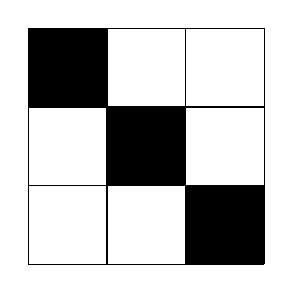
\begin{tikzpicture}
				\protect\fill (2,0) rectangle ++ (1,1); 
				\protect\fill (1,1) rectangle ++ (1,1); 
				\protect\fill (0,2) rectangle ++ (1,1); 
				\protect\draw (0,0) grid (3,3);
			\end{tikzpicture}}}

\begin{figure}[htb]
\begin{center}
\scalebox{0.625}{
\begin{tikzpicture}
\node[draw] (0) at (0,0) {\scalebox{.8}{$27 \hspace{1em} J=\emptyset  \hspace{1em} 0$}};
\node[draw] (3) at (-5,2.5) {\scalebox{.8}{
	\begin{tikzpicture}[anchor=south]
		\node (121a) at (0,1) {\scalebox{.5}{
			\begin{tikzpicture}
				\fill (2,0) rectangle ++ (1,1); 
				\fill (2,1) rectangle ++ (1,1); 
				\fill (2,2) rectangle ++ (1,1); 
				\draw (0,0) grid (3,3);
				\node (n) at (1.5,-1) {\scalebox{2}{$s_1s_2s_1$}};
			\end{tikzpicture}}};
		\node (txt) at (0,0) {$18 \hspace{1em} J=\{3\} \hspace{1em} 1$};
	\end{tikzpicture}}};
\node[draw] (2) at (0,2.5) {\scalebox{.8}{
	\begin{tikzpicture}[anchor=south]
		\node (13a) at (-2.2,1) {\scalebox{.5}{
			\begin{tikzpicture}
				\fill (0,0) rectangle ++ (1,1); 
				\fill (2,1) rectangle ++ (1,1); 
				\fill (1,2) rectangle ++ (1,1); 
				\draw (0,0) grid (3,3);
				\node (n) at (1.5,-1) {\scalebox{2}{$s_1s_3$}};
			\end{tikzpicture}}};
		\node (13b) at (0,1) {\scalebox{.5}{
			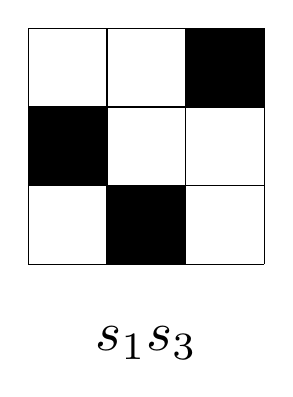
\begin{tikzpicture}
				\fill (1,0) rectangle ++ (1,1); 
				\fill (0,1) rectangle ++ (1,1); 
				\fill (2,2) rectangle ++ (1,1); 
				\draw (0,0) grid (3,3);
				\node (n) at (1.5,-1) {\scalebox{2}{$s_1s_3$}};
			\end{tikzpicture}}};
		\node (132) at (2.2,1) {\scalebox{.5}{
			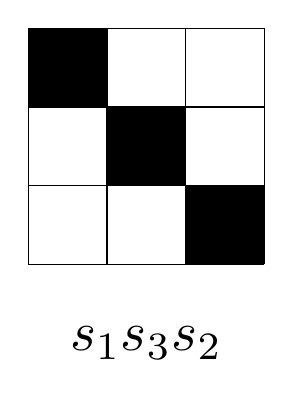
\begin{tikzpicture}
				\fill (2,0) rectangle ++ (1,1); 
				\fill (1,1) rectangle ++ (1,1); 
				\fill (0,2) rectangle ++ (1,1); 
				\draw (0,0) grid (3,3);
				\node (n) at (1.5,-1) {\scalebox{2}{$s_1s_3s_2$}};
			\end{tikzpicture}}};
		\node (txt) at (0,0) {$18 \hspace{1em} J=\{2\} \hspace{1em} 3$};
	\end{tikzpicture}}};
\node[draw] (1) at (5,2.5) {\scalebox{.8}{
	\begin{tikzpicture}[anchor=south]
		\node (232a) at (0,1) {\scalebox{.5}{
			\begin{tikzpicture}
				\fill (0,0) rectangle ++ (1,1); 
				\fill (0,1) rectangle ++ (1,1); 
				\fill (0,2) rectangle ++ (1,1); 
				\draw (0,0) grid (3,3);
				\node (n) at (1.5,-1) {\scalebox{2}{$s_2s_3s_2$}};
			\end{tikzpicture}}};
		\node (txt) at (0,0) {$18 \hspace{1em} J=\{1\} \hspace{1em} 1$};
	\end{tikzpicture}}};
\node[draw] (23) at (-7.5,7.5) {\scalebox{.8}{
	\begin{tikzpicture}[anchor=south]
		\node (1a) at (-2.2,1) {\scalebox{.5}{
			\begin{tikzpicture}
				\fill (0,0) rectangle ++ (1,1); 
				\fill (2,1) rectangle ++ (1,1); 
				\fill (1,2) rectangle ++ (1,1); 
				\draw (0,0) grid (3,3);
				\node (n) at (1.5,-1) {\scalebox{2}{$s_1$}};
			\end{tikzpicture}}};
		\node (1b) at (0,1) {\scalebox{.5}{
			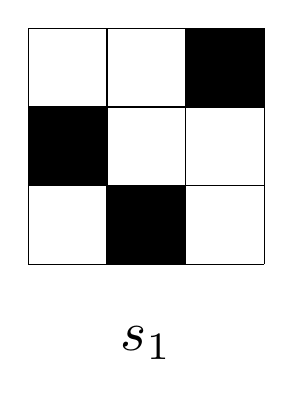
\begin{tikzpicture}
				\fill (1,0) rectangle ++ (1,1); 
				\fill (0,1) rectangle ++ (1,1); 
				\fill (2,2) rectangle ++ (1,1); 
				\draw (0,0) grid (3,3);
				\node (n) at (1.5,-1) {\scalebox{2}{$s_1$}};
			\end{tikzpicture}}};
		\node (1c) at (2.2,1) {\scalebox{.5}{
			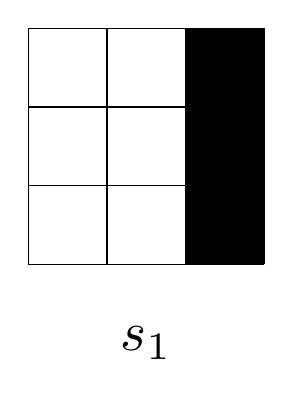
\begin{tikzpicture}
				\fill (2,2) rectangle ++ (1,1); 
				\fill (2,1) rectangle ++ (1,1); 
				\fill (2,0) rectangle ++ (1,1); 
				\draw (0,0) grid (3,3);
				\node (n) at (1.5,-1) {\scalebox{2}{$s_1$}};
			\end{tikzpicture}}};
		\node (12a) at (-1.2,3.5) {\scalebox{.5}{
			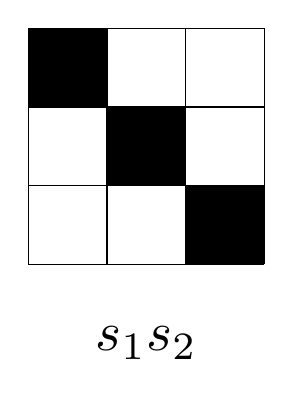
\begin{tikzpicture}
				\fill (0,2) rectangle ++ (1,1); 
				\fill (1,1) rectangle ++ (1,1); 
				\fill (2,0) rectangle ++ (1,1); 
				\draw (0,0) grid (3,3);
				\node (n) at (1.5,-1) {\scalebox{2}{$s_1s_2$}};
			\end{tikzpicture}}};
		\node (12b) at (1.2,3.5) {\scalebox{.5}{
			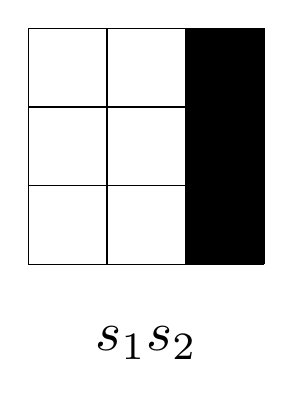
\begin{tikzpicture}
				\fill (2,0) rectangle ++ (1,1); 
				\fill (2,1) rectangle ++ (1,1); 
				\fill (2,2) rectangle ++ (1,1); 
				\draw (0,0) grid (3,3);
				\node (n) at (1.5,-1) {\scalebox{2}{$s_1s_2$}};
			\end{tikzpicture}}};
		\node (txt) at (0,0) {$10 \hspace{1em} J=\{2,3\} \hspace{1em} 5$};
	\end{tikzpicture}}};
\node[draw] (12) at (7.5,7.5) {\scalebox{.8}{
	\begin{tikzpicture}[anchor=south]
		\node (3a) at (2.2,1) {\scalebox{.5}{
			\begin{tikzpicture}
				\fill (0,0) rectangle ++ (1,1); 
				\fill (2,1) rectangle ++ (1,1); 
				\fill (1,2) rectangle ++ (1,1); 
				\draw (0,0) grid (3,3);
				\node (n) at (1.5,-1) {\scalebox{2}{$s_3$}};
			\end{tikzpicture}}};
		\node (3b) at (0,1) {\scalebox{.5}{
			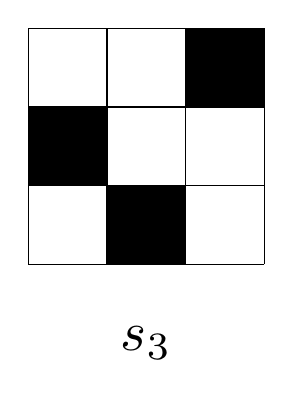
\begin{tikzpicture}
				\fill (1,0) rectangle ++ (1,1); 
				\fill (0,1) rectangle ++ (1,1); 
				\fill (2,2) rectangle ++ (1,1); 
				\draw (0,0) grid (3,3);
				\node (n) at (1.5,-1) {\scalebox{2}{$s_3$}};
			\end{tikzpicture}}};
		\node (3c) at (-2.2,1) {\scalebox{.5}{
			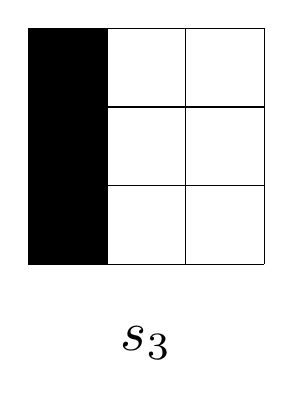
\begin{tikzpicture}
				\fill (0,2) rectangle ++ (1,1); 
				\fill (0,1) rectangle ++ (1,1); 
				\fill (0,0) rectangle ++ (1,1); 
				\draw (0,0) grid (3,3);
				\node (n) at (1.5,-1) {\scalebox{2}{$s_3$}};
			\end{tikzpicture}}};
		\node (32a) at (1.2,3.5) {\scalebox{.5}{
			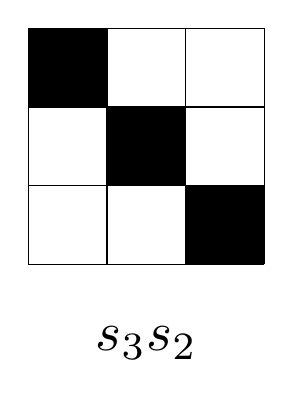
\begin{tikzpicture}
				\fill (0,2) rectangle ++ (1,1); 
				\fill (1,1) rectangle ++ (1,1); 
				\fill (2,0) rectangle ++ (1,1); 
				\draw (0,0) grid (3,3);
				\node (n) at (1.5,-1) {\scalebox{2}{$s_3s_2$}};
			\end{tikzpicture}}};
		\node (32b) at (-1.2,3.5) {\scalebox{.5}{
			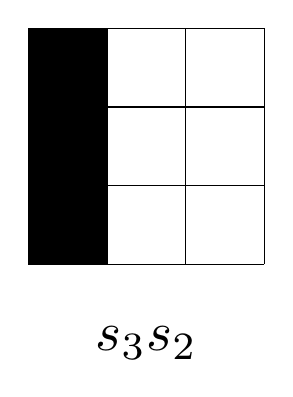
\begin{tikzpicture}
				\fill (0,0) rectangle ++ (1,1); 
				\fill (0,1) rectangle ++ (1,1); 
				\fill (0,2) rectangle ++ (1,1); 
				\draw (0,0) grid (3,3);
				\node (n) at (1.5,-1) {\scalebox{2}{$s_3s_2$}};
			\end{tikzpicture}}};
		\node (txt) at (0,0) {$10 \hspace{1em} J=\{1,2\} \hspace{1em} 5$};
	\end{tikzpicture}}};
\node[draw] (13) at (0,7.5) {\scalebox{.8}{
	\begin{tikzpicture}[anchor=south]
		\node (2a) at (2.2,1) {\scalebox{.5}{
			\begin{tikzpicture}
				\fill (0,0) rectangle ++ (1,1); 
				\fill (2,1) rectangle ++ (1,1); 
				\fill (1,2) rectangle ++ (1,1); 
				\draw (0,0) grid (3,3);
				\node (n) at (1.5,-1) {\scalebox{2}{$s_2$}};
			\end{tikzpicture}}};
		\node (2b) at (0,1) {\scalebox{.5}{
			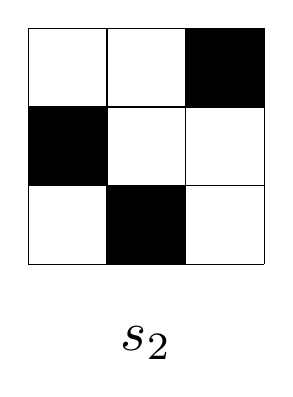
\begin{tikzpicture}
				\fill (1,0) rectangle ++ (1,1); 
				\fill (0,1) rectangle ++ (1,1); 
				\fill (2,2) rectangle ++ (1,1); 
				\draw (0,0) grid (3,3);
				\node (n) at (1.5,-1) {\scalebox{2}{$s_2$}};
			\end{tikzpicture}}};
		\node (2c) at (-2.2,1) {\scalebox{.5}{
			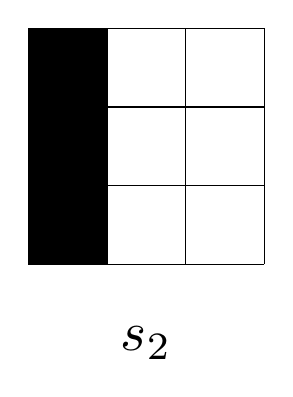
\begin{tikzpicture}
				\fill (0,2) rectangle ++ (1,1); 
				\fill (0,1) rectangle ++ (1,1); 
				\fill (0,0) rectangle ++ (1,1); 
				\draw (0,0) grid (3,3);
				\node (n) at (1.5,-1) {\scalebox{2}{$s_2$}};
			\end{tikzpicture}}};
		\node (23a) at (3.6,3.5) {\scalebox{.5}{
			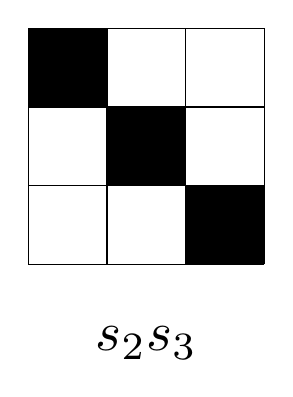
\begin{tikzpicture}
				\fill (0,2) rectangle ++ (1,1); 
				\fill (1,1) rectangle ++ (1,1); 
				\fill (2,0) rectangle ++ (1,1); 
				\draw (0,0) grid (3,3);
				\node (n) at (1.5,-1) {\scalebox{2}{$s_2s_3$}};
			\end{tikzpicture}}};
		\node (23b) at (1.2,3.5) {\scalebox{.5}{
			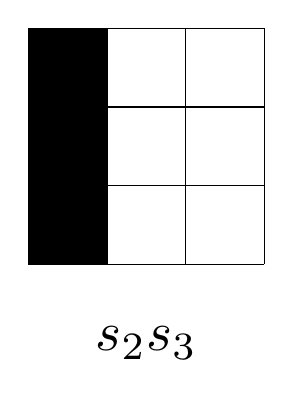
\begin{tikzpicture}
				\fill (0,0) rectangle ++ (1,1); 
				\fill (0,1) rectangle ++ (1,1); 
				\fill (0,2) rectangle ++ (1,1); 
				\draw (0,0) grid (3,3);
				\node (n) at (1.5,-1) {\scalebox{2}{$s_2s_3$}};
			\end{tikzpicture}}};
		\node (21a) at (-1.2,3.5) {\scalebox{.5}{
			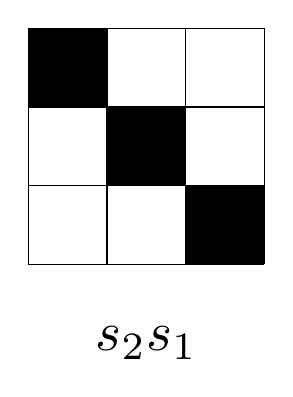
\begin{tikzpicture}
				\fill (0,2) rectangle ++ (1,1); 
				\fill (1,1) rectangle ++ (1,1); 
				\fill (2,0) rectangle ++ (1,1); 
				\draw (0,0) grid (3,3);
				\node (n) at (1.5,-1) {\scalebox{2}{$s_2s_1$}};
			\end{tikzpicture}}};
		\node (21b) at (-3.6,3.5) {\scalebox{.5}{
			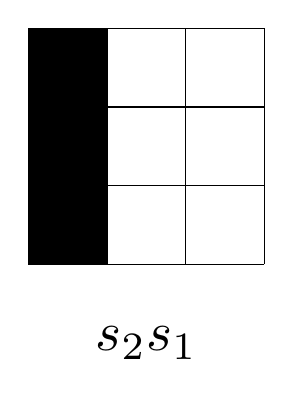
\begin{tikzpicture}
				\fill (0,0) rectangle ++ (1,1); 
				\fill (0,1) rectangle ++ (1,1); 
				\fill (0,2) rectangle ++ (1,1); 
				\draw (0,0) grid (3,3);
				\node (n) at (1.5,-1) {\scalebox{2}{$s_2s_1$}};
			\end{tikzpicture}}};
		\node (txt) at (0,0) {$12 \hspace{1em} J=\{1,3\} \hspace{1em} 7$};
	\end{tikzpicture}}};
	\node[draw] (123) at (0,12.5) {\scalebox{.8}{
	\begin{tikzpicture}[anchor=south]
		\node (ea) at (-6,1) {\scalebox{.5}{
			\begin{tikzpicture}
				\fill (0,0) rectangle ++ (1,1); 
				\fill (0,1) rectangle ++ (1,1); 
				\fill (0,2) rectangle ++ (1,1); 
				\draw (0,0) grid (3,3);
				\node (n) at (1.5,-1) {\scalebox{2}{$e$}};
			\end{tikzpicture}}};
		\node (eb) at (-3,1) {\scalebox{.5}{
			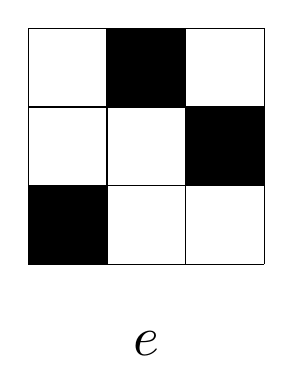
\begin{tikzpicture}
				\fill (0,0) rectangle ++ (1,1); 
				\fill (2,1) rectangle ++ (1,1); 
				\fill (1,2) rectangle ++ (1,1); 
				\draw (0,0) grid (3,3);
				\node (n) at (1.5,-1) {\scalebox{2}{$e$}};
			\end{tikzpicture}}};
		\node (ec) at (0,1) {\scalebox{.5}{
			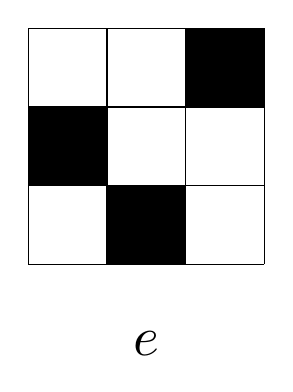
\begin{tikzpicture}
				\fill (1,0) rectangle ++ (1,1); 
				\fill (0,1) rectangle ++ (1,1); 
				\fill (2,2) rectangle ++ (1,1); 
				\draw (0,0) grid (3,3);
				\node (n) at (1.5,-1) {\scalebox{2}{$e$}};
			\end{tikzpicture}}};
		\node (ed) at (3,1) {\scalebox{.5}{
			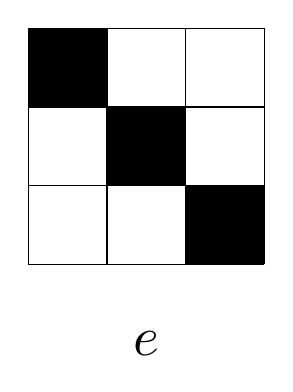
\begin{tikzpicture}
				\fill (2,0) rectangle ++ (1,1); 
				\fill (1,1) rectangle ++ (1,1); 
				\fill (0,2) rectangle ++ (1,1); 
				\draw (0,0) grid (3,3);
				\node (n) at (1.5,-1) {\scalebox{2}{$e$}};
			\end{tikzpicture}}};
		\node (ee) at (6,1) {\scalebox{.5}{
			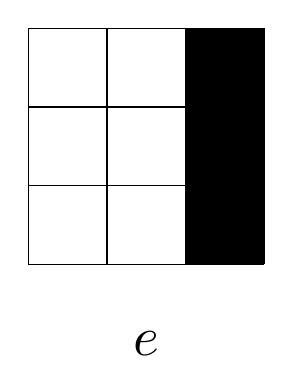
\begin{tikzpicture}
				\fill (2,0) rectangle ++ (1,1); 
				\fill (2,1) rectangle ++ (1,1); 
				\fill (2,2) rectangle ++ (1,1); 
				\draw (0,0) grid (3,3);
				\node (n) at (1.5,-1) {\scalebox{2}{$e$}};
			\end{tikzpicture}}};
		\node (txt) at (0,0) {$5 \hspace{1em} J=\{1,2,3\} \hspace{1em} 5$};
	\end{tikzpicture}}};
	\draw (0.north west) -- (3.south east);
	\draw (0.north east) -- (1.south west);
	\draw (0.north) -- (2.south);
	\draw (3.north east) -- (13.south west);
	\draw (3.north west) -- (23.south west);
	\draw (1.north west) -- (13.south east);
	\draw (1.north east) -- (12.south east);
	\draw (2.north west) -- (23.south east);
	\draw (2.north east) -- (12.south west);
	\draw (12.north east) -- (123.south east);
	\draw (13.north) -- (123.south);
	\draw (23.north west) -- (123.south west);
	%\draw (0) -- (2) -- (23);
	%\draw (0) -- (1) -- (12);
	%\draw (0) -- (1) -- (13);
\end{tikzpicture}}
\end{center}
\caption{We take $W = S_4$ and $\vec{c} = (s_1, s_2, s_3)$ and $\m = 3$.
Each box is a set $\mathcal{D}^J(\vec{c}^\m) \vcentcolon= \coprod_{v \in W^{J, +}} \mathcal{D}^{(v)}(\vec{c}^\m)$ for some $J$.
Edges between boxes are containments between $J$'s.
%A example of the parabolic parking objects as the maximal distinguished subwords of~\Cref{thm:parabolic1,thm:main} for $W=S_3$, $\m=3$, and $\vec{c}=(s_1,s_2,s_3)$.
Each $\vec{\omega} \in \mathcal{D}^J(\vec{c}^\m)$
% maximal distinguished subword 
is drawn as a $3 \times 3$ box, with skips $\omega^{(i)} = \id$ in black.
For example, \raisebox{-5pt}{\captionfig} represents $\vec{\omega} = (\id, s_2, s_3, s_1, \id, s_3, s_1, s_2, \id)$.
In each box, the number left, \emph{resp.}\@ right, of $J$ counts $w \in W$ with $\Des(w) \supseteq J$, \emph{resp.}\@ $\Des(w) = J$.
The former is $\Park_{W, \m}^{J, +}$.
% of maximal distinguished subwords for $v$ with descent set \emph{contained} in $S-J$ (resp. \emph{equal} to $S-J$).
The rightmost number in the $(k + 1)$th row is $\HOMFLYPT_{2k}(L_{4, 3})|_{\x \to 1}$.}
\label{fig:a3p3}
\end{figure}
%coefficients of HOMFLYPT at $q=1$ are recovered by the right-most $J$ in each row; the parabolic parking objects interpolate between parking objects (bottom) and Catalan objects (top).

%The image depicts all maximal distinguished subwords in $\bigsqcup_{J \subseteq S} \bigsqcup_{v \in W^J} \mathcal{M}^{(v)}(\vec{c}^\m)$.

By Theorem \ref{thm:trinh-parking}, the values $\CharQ{\mathbf{Z}(\vec{c}^\m)}(e_{S_n, \Lambda^k})$ for Coxeter words $\vec{c}$ and $\m$ coprime to $n$ are the \dfemph{rational $q$-Kirkman numbers} of~\cite{rss} in type $A$.
Via \eqref{eq:gltw}, Theorems \ref{thm:trinh-homflypt} and \ref{thm:asc} give:

\begin{cor}\label{cor:a-degree}
For any word $\vec{s} = (s_{i_1}, \ldots, s_{i_\ell})$ and $0 \leq k \leq n - 1$, we have
\begin{align}
\x^{\ell - n}
\HOMFLYPT_{2(n - 1 - k)}(L_{\beta_{\vec{s}}})
	= \frac{1}{(\x^2 - 1)^{n - 1}}
		\sum_{\substack{v \in S_n \\ \Des(v) = \{1, \ldots, k\}}}
		\sum_{\vec{\omega} \in \mathcal{D}^{(v)}(\vec{s})}
			\x^{2|\mathbf{d}_{\vec{\omega}}|} 
			(\x^2 - 1)^{|\mathbf{e}_{\vec{\omega}}|}.
\end{align}
That is, each $a$-degree of $\HOMFLYPT(L_{\beta_{\vec{s}}})$ is a sum of Deodhar-cell point counts.
\end{cor}

Figure \ref{fig:a3p3} illustrates Corollaries \ref{cor:parabolic} and \ref{cor:a-degree} simultaneously.
When $k = 0$, the outer sum on the right-hand side collapses to $v = \id$, and we recover the ``Legendrian ruling filtration'' formula of Shende--Treumann--Zaslow mentioned in \S\ref{subsec:geo}.

It is natural to seek a generalization of Corollary \ref{cor:a-degree} to other $W$.
For example, when $\vec{s} = \vec{c}^{h + 1}$, this would recover the $f$-vectors of the $W$-associahedron.
We have been unable to find such a construction.
This may be related to the absence of uniform formulas for $q$-Kirkman numbers in general.
Attractive formulas do exist for \dfemph{coincidental types}, where the degrees of $W$ form an arithmetic sequence \cite[\S{10}]{rss}.

%\section{Future Directions}\label{sec:future}

%Recall from classical combinatorics the important dichotomy between \emph{nonnesting} and \emph{noncrossing} partitions of $n$ objects.
%Both sets of partitions are counted by $\Cat_{n, n + 1}$.
%Nonnesting partitions generalize to sets depending on $\m$ and a root poset associated with $W$, whereas noncrossing partitions generalize to sets depending on $\m$ and a Coxeter word for $W$.
%An important open problem in Coxeter--Catalan combinatorics is to construct a bijection between a nonnesting family and a noncrossing family for $(W, \m)$, uniformly in $W$ and $\m$~\cite{williams}.

\acknowledgements{We thank our co-authors from~\cite{gltw}, P.\@ Galashin and T.\@ Lam, for helpful discussions.}

%% if you use biblatex then this generates the bibliography
%% if you use some other method then remove this and do it your own way
\printbibliography

\end{document}

 enumerative results generalizing those that involve the classical Catalan numbers, in two directions: a \emph{Coxeter} direction, depending on a finite, irreducible reflection group $W$; and a \emph{rational} direction, depending on an integer $\m > 0$ coprime to its Coxeter number

As we will explain in the last section, work of Sommers and others implicitly yields a nonnesting model for rational Coxeter--Catalan combinatorics in the algebraic geometry of affine Springer fibers.
We will present a complementary noncrossing model, in the geometry of so-called braid varieties.
